\documentclass[12pt]{article}
\usepackage{amsmath, amssymb, graphicx, hyperref}
\usepackage{listings}
\usepackage{xcolor}
\usepackage{caption}
\usepackage{geometry}
\usepackage{fancybox}
\usepackage{tcolorbox}
\geometry{margin=1in}

\title{Applying Edge Derivatives to Real-Time Object Detection}
\author{Valen Li}
\date{}

\begin{document}

\maketitle

\begin{abstract}
Edge derivatives --- the first and second partial derivatives of image intensity --- are fundamental to detecting object boundaries. Gradient-based filters (e.g., Sobel) and second-derivative filters (e.g., Laplacian) measure sharp intensity changes, revealing edges. In practice, these operators are used to create binary masks of object silhouettes or support region proposals in real-time detection pipelines. OpenCV provides optimized functions for these tasks (e.g., \texttt{cv2.Sobel}, \texttt{cv2.Canny}, \texttt{cv2.findContours}). I present the mathematical foundations of image derivatives, describe how they highlight boundaries, and survey their role in object detection and masking. I detail common OpenCV implementations and illustrate with code. 
\end{abstract}

\section{Introduction}
Edges in images correspond to object boundaries or transitions between regions. Formally, edges are locations of rapid intensity change, which can be detected by computing image derivatives. The image gradient \( \nabla I = \left( \frac{\partial I}{\partial x}, \frac{\partial I}{\partial y} \right) \) encodes the direction and magnitude of maximal change. High gradient magnitude typically indicates an object contour. Thus, edge detection --- finding pixels where \( \|\nabla I\| \) is large --- is a cornerstone of image processing and object recognition.

Traditional pipelines blur an image to reduce noise, compute gradients (via Sobel or Prewitt filters), and threshold the gradient magnitude to obtain an edge map. These edges are used to build binary masks or proposals that guide object detection.

OpenCV offers efficient implementations of these operators, enabling real-time use. Functions like \texttt{cv2.Sobel()} and \texttt{cv2.Canny()} compute derivatives and edge maps on-the-fly, and \texttt{cv2.findContours()} extracts continuous boundary curves from binary masks. 

\section{Mathematical Overview of Edge Derivatives}
An image is a discrete sampling of a continuous intensity function. The first partial derivatives \( \frac{\partial I}{\partial x} \) and \( \frac{\partial I}{\partial y} \) measure intensity change along horizontal and vertical axes. The gradient vector points in the direction of greatest increase, and its magnitude is

\[ \|\nabla I\| = \sqrt{\left(\frac{\partial I}{\partial x}\right)^2 + \left(\frac{\partial I}{\partial y}\right)^2} \]

In practice, these derivatives are approximated by convolution with discrete kernels. A common choice is the Sobel operator. For example, the horizontal and vertical Sobel kernels are:

\[
G_x = \begin{bmatrix}-1 & 0 & 1 \\ -2 & 0 & 2 \\ -1 & 0 & 1\end{bmatrix}, \quad G_y = \begin{bmatrix}-1 & -2 & -1 \\ 0 & 0 & 0 \\ 1 & 2 & 1\end{bmatrix}
\]

Convolving an image \( I \) with \( G_x \) and \( G_y \) gives approximations of \( \frac{\partial I}{\partial x} \) and \( \frac{\partial I}{\partial y} \), respectively. These can be combined into the gradient magnitude:

\[ \|\nabla I\| = \sqrt{(G_x * I)^2 + (G_y * I)^2} \]

Applying the Sobel filter to a real image produces an edge map highlighting object outlines. 


\begin{figure}[h!]
    \centering
    \begin{tcolorbox}[colframe=black!80, colback=white, boxrule=0.5mm, arc=6pt, width=0.65\textwidth]
        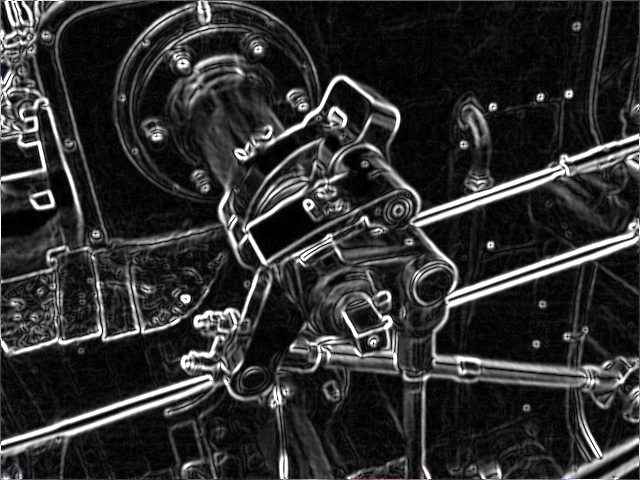
\includegraphics[width=\linewidth]{sobel_edge_detection_example.png}
    \end{tcolorbox}
    \label{fig:sobel}
\end{figure}

Beyond first derivatives, the Laplacian operator (sum of second partials) is \( \nabla^2 I = \frac{\partial^2 I}{\partial x^2} + \frac{\partial^2 I}{\partial y^2} \), also used for edge detection. The Laplacian responds strongly at points of rapid second-order change (e.g. zero-crossings at edges). In OpenCV, cv2.Laplacian() implements this second-derivative filter,
though in many pipelines first-derivative methods (Sobel, Canny) are preferred due to noise sensitivity of second derivatives.

\section{Edge Maps for Object Boundary Detection}
Edges detected via derivatives often coincide with object boundaries. In an image, boundaries between objects or regions produce sharp intensity changes; thus gradient magnitudes peak along contours. By thresholding the gradient (or finding zero-crossings of second derivatives), one obtains a binary edge map outlining objects. For instance, the Canny edge detector uses Sobel gradients plus non-maximum suppression and dual thresholds to yield thin edges along true boundaries. In all cases, the core step is the same: highlight pixels where $\|\nabla I\|$ is large or where $\nabla^2 I$ changes sign.

Once an edge map is obtained, contour detection or mask creation can follow. A contour is formally a connected curve of constant intensity (often along an edge). OpenCV defines contours as continuous boundary points of objects. In practice one typically creates a binary (white-on-black) image of edges or object regions, then calls \texttt{cv2.findContours()} to extract contour curves. These contours can be analyzed to find object shapes or to fit bounding boxes. In fact, OpenCV’s documentation notes that:

\begin{quote}
“Contours can be explained simply as a curve joining all the continuous points along the boundary having the same color or intensity. The contours are a useful tool for shape analysis and object detection and recognition.”
\end{quote}

It also recommends using thresholding or Canny before \texttt{findContours()} to generate a clean binary image.

Thus, a typical edge-based segmentation pipeline is:
\begin{itemize}
\item \textbf{Smoothing}: Blur the image (e.g., Gaussian) to reduce noise.
\item \textbf{Gradient computation}: Use Sobel/Canny to compute $\partial I / \partial x$, $\partial I / \partial y$, and form an edge map.
\item \textbf{Thresholding}: Binarize the edge map (e.g., via hysteresis thresholds in Canny, or a fixed threshold on $\| \nabla I \|$).
\item \textbf{Morphological closing (optional)}: Dilate/erode to connect edge fragments.
\item \textbf{Contour detection}: Use \texttt{cv2.findContours()} on the binary mask to extract object boundaries.
\item \textbf{Mask generation}: Fill or draw contours to create object masks or bounding boxes for detection.
\end{itemize}

These steps turn low-level edge derivatives into higher-level region masks or bounding boxes. For example, in moving-object detection one common pipeline is background subtraction followed by contour extraction. Similarly, a static image pipeline might simply run Canny on each frame and extract contours. The contours (or their bounding boxes) are then fed to a recognition module (e.g., a classifier or a deep CNN) for final object identification.

\section{Role of Edges and Masking in Real-Time Detection}
One use for edges is masking. For tasks like instance segmentation or focused detection, one may compute an edge-derived mask of the foreground. For example, one can detect edges, fill closed contours, and treat the result as a foreground mask. This mask can suppress the background and limit the detector’s search region. In video applications, background subtraction + contours (essentially an edge-based mask) is often used for “moving object detection”. Here, contours outline the moving objects, and those outlines define masks or bounding boxes for tracking. In some systems (e.g. robotics), an edge mask is even used as a prior to guide a CNN’s attention or a CRF post-processing step.


\section{OpenCV Functions and Code Snippets}
Important OpenCV functions include:
\begin{itemize}
\item \texttt{cv2.Sobel(src, ddepth, dx, dy, ksize)}: Computes first-order derivatives. For example, \texttt{cv2.Sobel(img, cv2.CV\_64F, 1, 0, ksize=3)} yields $\frac{\partial I}{\partial x}$ ; swapping \texttt{dx=0, dy=1} gives . The outputs can be combined to form edge magnitudes.
\item \texttt{cv2.Laplacian(src, ddepth, ksize)}: Computes the Laplacian \( \nabla^2 I \), using a discrete kernel (e.g., 3×3 or 5×5). Useful for zero-crossing edge detection, often applied after Gaussian smoothing.

\item \texttt{cv2.Canny(image, threshold1, threshold2)}: A complete edge detector that includes Gaussian blur, Sobel gradient, non-maximum suppression, and double-threshold hysteresis. Returns a binary edge map. Canny is widely used for real-time edges due to its good noise tolerance.

\item \texttt{cv2.threshold(src, thresh, maxval, type)}: Produces a binary image by thresholding pixel intensities. Often used to binarize gradient magnitude or grayscale images before contour finding.

\item \texttt{cv2.findContours(image, mode, method)}: Extracts contours from a binary image. For example, \texttt{contours,\_ = cv2.findContours(edges, cv2.RETR\_EXTERNAL, cv2.CHAIN\_APPROX\_SIMPLE)}. OpenCV documentation notes that input should be binary (e.g., after thresholding or Canny).

\item \texttt{cv2.drawContours}, \texttt{cv2.boundingRect}: Used to draw or bound the detected contours. One might loop through each contour, compute its bounding box, and draw it on the original image.
\end{itemize}

Example pipeline:
\begin{verbatim}
import cv2
import numpy as np

# Read image or video frame (BGR)
frame = cv2.imread('frame.jpg')

# 1. Preprocess: convert to grayscale and blur
gray = cv2.cvtColor(frame, cv2.COLOR_BGR2GRAY)
gray = cv2.GaussianBlur(gray, (3,3), 0)

# 2. Edge detection: Canny for a binary edge map
edges = cv2.Canny(gray, 100, 200)

# 3. Find contours on the edge mask
contours = cv2.findContours(edges, cv2.RETR_EXTERNAL, cv2.CHAIN_APPROX_SIMPLE)

# 4. Draw bounding boxes around each contour
for cnt in contours:
    x, y, w, h = cv2.boundingRect(cnt)
    cv2.rectangle(frame, (x, y), (x+w, y+h), (0, 255, 0), 2)

# 5. Display or further process frame with detections
cv2.imshow('Edges', edges)
cv2.imshow('Detections', frame)
cv2.waitKey(0)
\end{verbatim}

This snippet demonstrates a simple pipeline: computing edges with \texttt{cv2.Canny} and then extracting bounding boxes via \texttt{cv2.findContours} and \texttt{cv2.boundingRect}. In practice, one might refine the mask (e.g., dilation to close gaps) or filter contours by area to remove noise.

Other variants could use \texttt{cv2.Sobel()} directly to compute gradients and then threshold the magnitude:

\begin{verbatim}
# Compute Sobel gradients
sobelx = cv2.Sobel(gray, cv2.CV_64F, 1, 0, ksize=3)
sobely = cv2.Sobel(gray, cv2.CV_64F, 0, 1, ksize=3)

# Compute gradient magnitude
mag = cv2.magnitude(sobelx, sobely)
mag = np.uint8(np.clip(mag, 0, 255))

# Threshold to binary mask
mask = cv2.threshold(mag, 50, 255, cv2.THRESH_BINARY)

# Extract contours
contours = cv2.findContours(mask, cv2.RETR_EXTERNAL, cv2.CHAIN_APPROX_SIMPLE)
\end{verbatim}

Here, \texttt{cv2.magnitude} combines G\_x and G\_y into $||\nabla I|| $, then a threshold yields a mask. Regardless of method, the role of these derivatives is to produce a mask aligned with object edges.


\section{Summary}
Edge derivatives (gradients and Laplacians) provide a mathematically grounded way to detect abrupt intensity changes --- typically object boundaries. In OpenCV, functions like \texttt{cv2.Sobel} and \texttt{cv2.Canny} compute these derivatives efficiently. The resulting edge maps can be converted into binary masks and contours (via \texttt{cv2.findContours}) which isolate objects for detection or segmentation.

\subsection*{Key Functions and Equations}
\begin{itemize}
\item The image gradient $\nabla I = (\partial I/\partial x, \partial I/\partial y)$ is approximated by Sobel kernels.
\item The gradient magnitude $\|\nabla I\| = \sqrt{(\partial I/\partial x)^2 + (\partial I/\partial y)^2}$ identifies edges.
\item The Laplacian $\nabla^2 I = \partial^2 I/\partial x^2 + \partial^2 I/\partial y^2$ can also detect edges via zero-crossings.
\item OpenCV implements these via \texttt{cv2.Sobel}, \texttt{cv2.Laplacian}, and the popular \texttt{cv2.Canny} edge detector.
\item After obtaining a binary edge mask, one uses \texttt{cv2.findContours} to extract object boundaries.
\end{itemize}

This pipeline of derivative  mask  contour provides the basis for many real-time object detection systems.

\newpage
\section{Sources}
\begin{itemize}

\item \url{https://en.wikipedia.org/wiki/Laplace_operator}
\item \url{https://en.wikipedia.org/wiki/Sobel_operator#:~:text=Image%3A%20,2}
\item \url{https://www.geeksforgeeks.org/real-time-edge-detection-using-opencv-python/}
\item \url{https://www.cs.cornell.edu/courses/cs664/2003fa/handouts/664-l6-edges-03.pdf#:~:text=%C2%83%20Idealized%20continuous%20image%20I,%E2%88%82I%2F%20%E2%88%82x%2C%20%E2%88%82I%2F%20%E2%88%82y}
\item \url{https://docs.opencv.org/3.4/d4/d73/tutorial_py_contours_begin.html#:~:text=Contours%20can%20be%20explained%20simply,and%20object%20detection%20and%20recognition}
\item \url{https://paperswithcode.com/dataset/coco#:~:text=The%20MS%20,of%20the%202015%20test%20set}
\item \url{https://learnopencv.com/edge-detection-using-opencv/#:~:text=Edge%20detection%20is%20an%20image,use%20edge%20detection%20in%20applications}
\item \url{https://blog.roboflow.com/edge-detection/#laplacian-edge-detection}
\item \url{https://github.com/matterport/Mask_RCNN/releases}
\item \url{https://www.analyticsvidhya.com/blog/2019/07/computer-vision-implementing-mask-r-cnn-image-segmentation/}
\end{itemize}

\end{document}
